\subsection{Odometry parameters}
\label{sse:odometry_single_plane_params}

\subsubsection{The {\tt Rox\_Odometry\_Params} object}
\label{sss:odometry_single_plane_params_object}

A \lstinline$Rox_Odometry_Single_Plane_Params$ object can be defined using the pointer to a \lstinline$Rox_Tracking_Params_Structure$:
\begin{lstlisting}
typedef struct Rox_Tracking_Params_Struct* Rox_Odometry_Single_Plane_Params;
\end{lstlisting}
The structure is opaque to the users.

\subsubsection{Creating/Deleting a {\tt Rox\_Odometry\_Params}}
\label{sss:odometry_single_plane_params_newdel}

Functions are provided to allocate and deallocate a \lstinline$Rox_Odometry_Single_Plane_Params$ object~:

\begin{lstlisting}
Rox_Error rox_odometry_single_plane_params_new (Rox_Odometry_Single_Plane_Params *params);
\end{lstlisting}
The \lstinline$rox_odometry_single_plane_params_new$ function allocates memory for the odometry object and returns a pointer on the newly created object.

\begin{lstlisting}
Rox_Error rox_odometry_single_plane_params_del (Rox_Odometry_Single_Plane_Params *params);
\end{lstlisting}
The function deallocates memory for a \lstinline$Rox_Odometry_Single_Plane_Params$ object. It is necessary to call this function when the object is not used anymore. \\

\subsubsection{Main functions related to {\tt Rox\_Odometry\_Params}}
\label{sss:odometry_single_plane_params_methods}

% \paragraph{Localization relative to objects with known size}
% \label{par:odometry_model}
% ~\\~\\
The camera localization is done relative to a known object. It is
assumed that a rectangular planar object with size (sizx, sizy) is
observed. In this case it is possible to know the pose of the camera
relative to the planar object (the object frame is centered on the
rectangular object, see figure~\ref{model_size}) and also the
displacement of the camera between two images.

\begin{figure}[htbp] 
\begin{center}
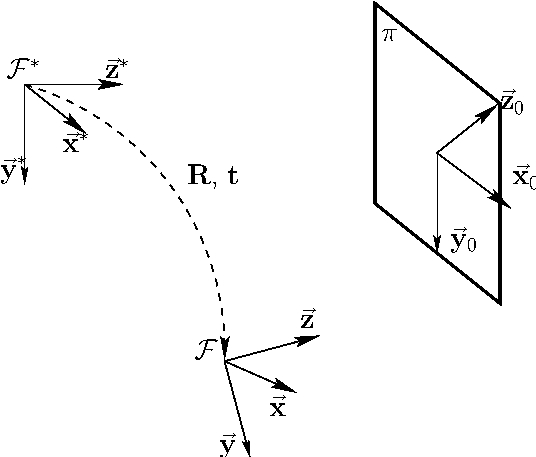
\includegraphics[width=0.75\textwidth]{odometry/figures/model_size}
\caption{Localization relative to a planar object with known size.}
\label{model_size}
\end{center}
\end{figure}

% \paragraph{Localization relative to objects with known normal}
% \label{par:odometry_scale}
% ~\\~\\
% If the camera localization is done relative to a known object the user shall set the scaled normal of the plane using the following function:

% \begin{lstlisting}
% Rox_Void rox_odometry_single_plane_params_set_model_normal(Rox_Odometry_Single_Plane_Params P, Rox_Vector nd)
% \end{lstlisting}

% \begin{figure}[htbp] 
% \begin{center}
% 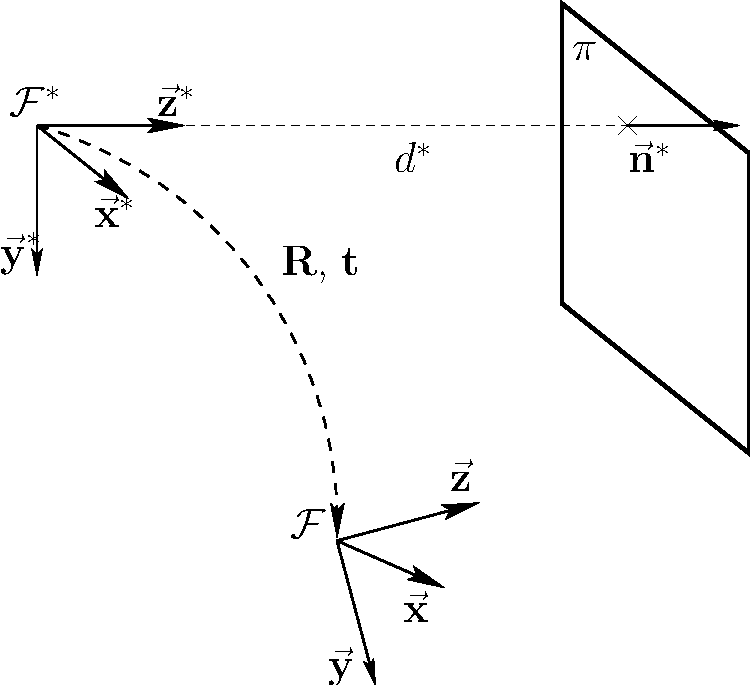
\includegraphics[width=0.5\textwidth]{odometry/figures/model_norm}
% \caption{Localization relative to a planar object with unknown size.}
% \label{model_norm}
% \end{center}
% \end{figure}

